
\section{Générateur de marche en boucle ouverte et stabilisation\label{sec:walk}}

Le mouvement de marche\footnote{Le code open source C++ 
de l'implémentation du générateur de marche utilisé par les robots Sigmaban
est disponible à l'adresse suivante : \url{https://github.com/rhoban/ikwalk}}
détaillé ici est utilisé par les robots humanoïdes de l'équipe Rhoban 
depuis la participation à la RoboCup 2014.
Il a été présenté à la communauté RoboCup dans 
l'article \cite{ProjectsWorkshopHumanoids2015}.
Ce mouvement de marche se base sur d'une part, la génération de trajectoires
de références en boucle ouverte dans l'espace cartésien (module appelé \textit{IKWalk})
ainsi que sur une boucle de stabilisation utilisant les capteurs
de pression des pieds du robot.

\subsection{Description du générateur}

\begin{table}[htbp]
\begin{center}
    \begin{tabular}{|p{3.5cm}|p{6cm}|p{1.5cm}|c|l|}
        \hline
        Paramètre statique & Description & Valeur typique & Unité & Bornes\\
        \hline
        \textit{freq} & 
            Fréquence d'un cycle complet de marche (deux pas). & 
            $1.7$ & Hz & $[1,2]$\\
        \textit{footYOffset} & 
            Distance latérale statique entre les deux pieds. & 
            $0.025$ & m & $[0.02, 0.04]$\\
        \textit{riseGain} & 
            Hauteur de levée des pieds. & 
            $0.035$ & m & $[0,0.05]$\\
        \textit{swingGain} & 
            Amplitude des oscillations latérales du buste par rapport aux pieds. & 
            $0.02$ & m & $[0,0.04]$\\
        \textit{swingPhase} & 
            Décalage de phase des oscillations latérales du buste. & 
            $0.25$ & phase & $[0,1]$\\
        \textit{trunkXOffset} & 
            Décalage statique avant/arrière de la position du buste par rapport aux pieds. & 
            $0.01$ & m & $[-0.03,0.03]$\\
        \textit{trunkYOffset} & 
            Décalage statique latéral de la position du buste par rapport aux pieds. & 
            $0.0$ & m & $[-0.02,0.02]$\\
        \textit{trunkZOffset} & 
            Décalage en hauteur statique du buste par rapport à la hauteur initiale jambes tendues. & 
            $0.02$ & m & $[0.005,0.04]$\\
        \textit{trunkPitch} & 
            Inclinaison avant/arrière du buste. & 
            $0.2$ & radian & $[0,0.25]$\\
        \textit{trunkRoll} & 
            Inclinaison latérale du buste. & 
            $0.0$ & radian & $[-0.1, 0.1]$\\
        \textit{swingVel} & 
            Vitesse latérale du buste au changement de support. & 
            $4.0$ & m.s$^{-1}$ & \\
        \textit{stepUpVel} & 
            Vitesse du pied vers l'avant à la fin de la phase de support. &
            $5.0$ & m.s$^{-1}$ & $[0,5]$\\
        \textit{stepDownVel} & 
            Vitesse du pied vers l'arrière au début de la phase de support. &
            $5.0$ & m.s$^{-1}$ & $[0,5]$\\
        \textit{riseUpVel} & 
            Vitesse du pied vers le haut à la fin de la phase de support. & 
            $5.0$ & m.s$^{-1}$ & $[0,5]$\\
        \textit{riseDownVel} & 
            Vitesse du pied vers le bas au début de la phase de support. & 
            $5.0$ & m.s$^{-1}$ & $[0,5]$\\
        \hline
    \end{tabular}
    \caption{\label{tab:walk_params_static}Liste des paramètres statiques 
    du mouvement de marche en boucle ouverte \textit{IKWalk}.}
\end{center}
\end{table}
\begin{table}[htb!]
\begin{center}
    \begin{tabular}{|l|p{5cm}|p{1.5cm}|c|l|}
        \hline
        Paramètre dynamique & Description & Valeur typique & Unité & Bornes\\
        \hline
        \textit{enabledGain} & 
            Coefficient se multipliant sur toutes les parties oscillantes.
            0 : arrête la marche. 1 : amplitudes complètes. & 
            $1.0$ & 1 & $[0,1]$\\
        \textit{stepGain} & 
            Longueur des pas dans la direction avant/arrière. &
            $0.04$ & m & $[-0.05,0.05]$\\
        \textit{lateralGain} & 
            Longueur des pas latéraux. & 
            $0.01$ & m & $[-0.02,0.02]$\\
        \textit{turnGain} & 
            Angle de la rotation des pieds à chaque pas. & 
            $0.1$ & radian & $[-0.26,0.26]$\\
        \hline
    \end{tabular}
    \caption{\label{tab:walk_params_dynamic}Liste des paramètres dynamiques 
    du mouvement de marche en boucle ouverte \textit{IKWalk}.}
\end{center}
\end{table}

Le générateur \textit{IKWalk} est un mouvement de marche avec 
les caractéristiques suivantes :
\begin{itemize}
    \item Le mouvement est configuré et contrôlé au travers de paramètres.
        Le réglage manuel de ces paramètres par expérimentations directes sur 
        le robot réel assure la stabilité 
        du système\footnote{Le mouvement de marche se repose en très grande 
        partie sur stabilité mécanique naturel du système.}.
    \item Le mouvement est en boucle ouverte. 
        L'état du mouvement est entièrement déterminé par sa phase 
        (ou affixe) ainsi que par la valeur courante des paramètres.
        En fixant les ordres de la marche, la commande de toutes 
        les articulations est périodique.
    \item La marche est omnidirectionnelle. 
        Le robot doit être capable de se déplacer sur le sol dans toutes
        les directions en plus de pouvoir tourner sur lui même.
        Mathématiquement, la description de l'état du robot sur le
        sol fait intervenir trois dimensions : 
        $\begin{bmatrix}x & y & \theta\end{bmatrix}^{\mathsf{T}}$.
        Le mouvement fait appel à des mélanges de pas dans la direction 
        avant arrière ainsi que des pas latéraux (pas chassés).
        Le déplacement est contrôlé en vitesse au travers de trois paramètres dynamiques :\\
        $\begin{bmatrix}\text{\textit{stepGain}} & \text{\textit{lateralGain}} 
        & \text{\textit{turnGain}}\end{bmatrix}^{\mathsf{T}}$\\
        Ces paramètres représentent la longueur et la rotation de chaque pas.
    \item Le générateur exprime les trajectoires cartésiennes 
        désirées des pieds dans le repère du tronc. 
        Les commandes moteurs sont alors calculées au travers du 
        modèle géométrique inverse (voir section \ref{sec:modele_inverse}) 
        des deux jambes.
\end{itemize}

Plus formellement, le générateur se 
représente par la fonction suivante :
$$
\mathsf{IKWalk} : 
\big(\Delta t, \varphi_{t}, \bm{\theta}_{\text{statique}}, \bm{\theta}_{\text{dynamique}}\big) 
\longmapsto 
\big(\bm{q}_{\text{référence}}, \varphi_{t+1}\big)
$$
$\varphi_{t} \in [0,1[$ est la phase courante ou l'avancement dans le cycle du mouvement.
La fonction calcule et renvoie la phase suivante $\varphi_{t+1}$ à partir de $\varphi_{t}$,
du temps $\Delta t$ écoulé depuis le dernier appel à la fonction et de la fréquence de la 
marche (qui est un élément de $\bm{\theta}_{\text{statique}}$).
$\bm{\theta}_{\text{statique}} \in \mathbb{R}^{n}$ et $\bm{\theta}_{\text{dynamique}} \in \mathbb{R}^{m}$ 
sont les vecteurs des paramètres statiques et dynamiques énumérés dans 
les tableaux \ref{tab:walk_params_static} et \ref{tab:walk_params_dynamic} permettant
de configurer la marche.
Enfin, la fonction calcule et retourne la position cible de toutes les articulations 
dans le vecteur $\bm{q}_{\text{référence}}$.

La phase $\varphi_{t}$ augmente strictement au cours du mouvement
dans l'intervalle \textbf{circulaire} $[0,1[$. La convention suivante est adoptée :
\begin{itemize}
    \item En $\varphi_{t} = 0$, le pied gauche se pose et 
        la phase de support gauche commence. 
        Le pied droit décolle et la phase de support droit se termine.
    \item En $\varphi_{t} = 0.5$, le pied gauche décolle et 
        la phase de support gauche se termine. 
        Le pied droit se pose et la phase de support droit commence.
\end{itemize}
Les paramètres \textit{statiques} (tableau \ref{tab:walk_params_static}) 
ne sont pas mis à jour pendant le mouvement et sont
réglés manuellement par expérimentation sur le robot.
L'objectif recherché est d'assurer la stabilité du robot 
sous différents ordres et de maximiser la vitesse de déplacement maximale. 
Les paramètres \textit{dynamiques} (tableau \ref{tab:walk_params_dynamic}) sont quant
à eux les \textit{ordres} en vitesse de la marche. 
Ils sont continuellement modifiés afin de contrôler la direction du déplacement.
Plus précisément, les paramètres dynamiques 
(\textit{stepGain}, \textit{lateralGain} et \textit{turnGain}) 
ne sont réellement mis à jour qu'au moment du changement de pied du 
support (à $\varphi = 0$ et $0.5$).
Un pas du robot (un demi cycle de marche) est donc bien défini
par son déplacement en $\bm{\vec{x}},\bm{\vec{y}}$ et sa rotation.\\

Au démarrage et à l'arrêt du mouvement de marche, un lissage
est effectué afin d'améliorer la stabilité et de laisser le temps
au robot d'entrer en oscillation.
Le paramètre dynamique \textit{enableGain} passe progressivement de
$0$ à $1$ et permet d'augmenter lentement l'amplitude
de toutes les oscillations cartésiennes.

Enfin, il s'avère que les changements d'ordres brutaux de la marche
tendent parfois à déstabiliser le robot.
Notamment lorsque de forts ordres d'avance, de pas latéraux 
et de rotations sont demandés.
Une limite en accélération est alors fixée afin de tenir compte
des effets de l'inertie.
Il s'agit donc d'une borne sur les variations de chacune 
des trois dimension des ordres de la marche.
Le réglage de ces seuils est réalisé en même temps que l'ajustement
manuel des paramètres statiques du mouvement.
À noter que ces limites d'accélération rendent plus difficile
la planification de l'approche évoquée à la section \ref{sec:odometry_mdp}.

\subsection{Principe de fonctionnement du générateur}

Le but du générateur de marche est de fixer dans
le repère du buste du robot (\textit{trunk}) la position
et l'orientation souhaitées du centre des pieds 
(\textit{left\_foot\_tip}, \textit{right\_foot\_tip}) correspondant 
à la phase $\varphi_{t}$ courante du mouvement.
Dans un second temps, les positions cibles de toutes les
articulations du robot sont calculées au travers du modèle 
géométrique inverse des jambes et envoyées aux moteurs.
Le calcul des positions et orientations cartésiennes désirées
se base sur les quatre splines polynomiales cubiques représentées 
sur le graphique \ref{fig:walk_splines}.
Ces splines normalisées représentent la forme des oscillations cartésiennes. 
Les paramètres statiques et dynamiques du mouvement sont ensuite utilisés pour 
multiplier l'amplitude, décaler et selon les cas déphaser ces oscillations
pour engendrer les trajectoires souhaitées.
Les splines sont exprimées par convention pour le pied
gauche. Un décalage de phase de $0.5$ (un demi cycle) est appliqué 
lors de l'évaluation des splines pour le pied droit :
\begin{description}
    \item[\textit{rise}] Représente la hauteur des pieds. 
        Pendant la phase de support, le pied est sur le sol 
        puis il s'élève et se repose.
    \item[\textit{step}] Représente le mouvement avant arrière des pieds selon $\bm{\vec{x}}$.
        À noter que le mouvement des pas latéraux utilise aussi cette spline.
    \item[\textit{swing}] Représente la translation latérale du buste par 
        rapport aux pieds, utilisée pour déporter le poids du robot.
        Le haut du corps oscille de gauche à droite. 
        Le poids du corps est à droite ($y$ négatifs) au moment où le pied gauche est en l'air.
        Cette spline est la seule à être déphasée (\textit{swingPhase}).
    \item[\textit{turn}] Représente l'angle des pieds par rapport à 
        $\bm{\vec{x}}$ (repère égocentrique) lorsqu'un ordre en rotation est donné.
        Le pied tourne dans un sens pendant la phase de support 
        et tourne dans l'autre sens pendant la phase de vol.
\end{description}

Le schéma \ref{fig:walk_schema} résume l'architecture général du générateur.
Le calcul complet de toutes les positions cibles cartésiennes n'est pas 
détaillé ici mais peut être retrouvé dans 
l'implémentation \textit{open-source}.
Néanmoins, l'exemple suivant montre le calcul de la hauteur $h$ des
pieds gauche et droit dans le repère du buste :
$$
h_{\text{pied gauche}} = 
\text{\textit{enableGain}}~.~\text{\textit{riseGain}}~.~\mathsf{spline}_{\text{\textit{rise}}}(\varphi_{t})
- \text{\textit{trunkZOffset}}
+ \text{\textit{legLength}}
$$
$$
h_{\text{pied droit}} = 
\text{\textit{enableGain}}~.~\text{\textit{riseGain}}~.~\mathsf{spline}_{\text{\textit{rise}}}(\varphi_{t}+0.5)
- \text{\textit{trunkZOffset}}
+ \text{\textit{legLength}}
$$
où $\textit{legLength}$ est la distance entre le buste et le centre 
des pieds jambes tendues (degrés de liberté en zéro)

\begin{figure}[htb]
    \begin{center}
        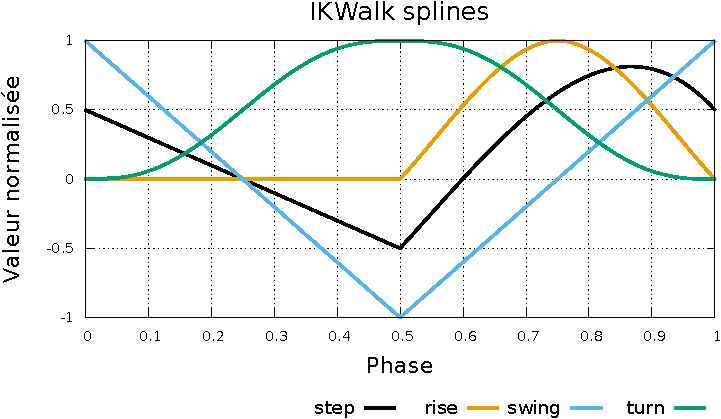
\includegraphics[type=pdf,ext=.pdf,read=.pdf,width=0.95\linewidth]{../plot/walk_splines}
        \caption{\label{fig:walk_splines} 
            Les quatre splines cubiques périodiques à la base des mouvements 
            cartésiens oscillant du générateur de marche IKWalk.}
    \end{center}
\end{figure}

\begin{figure}[htb]
    \begin{center}
        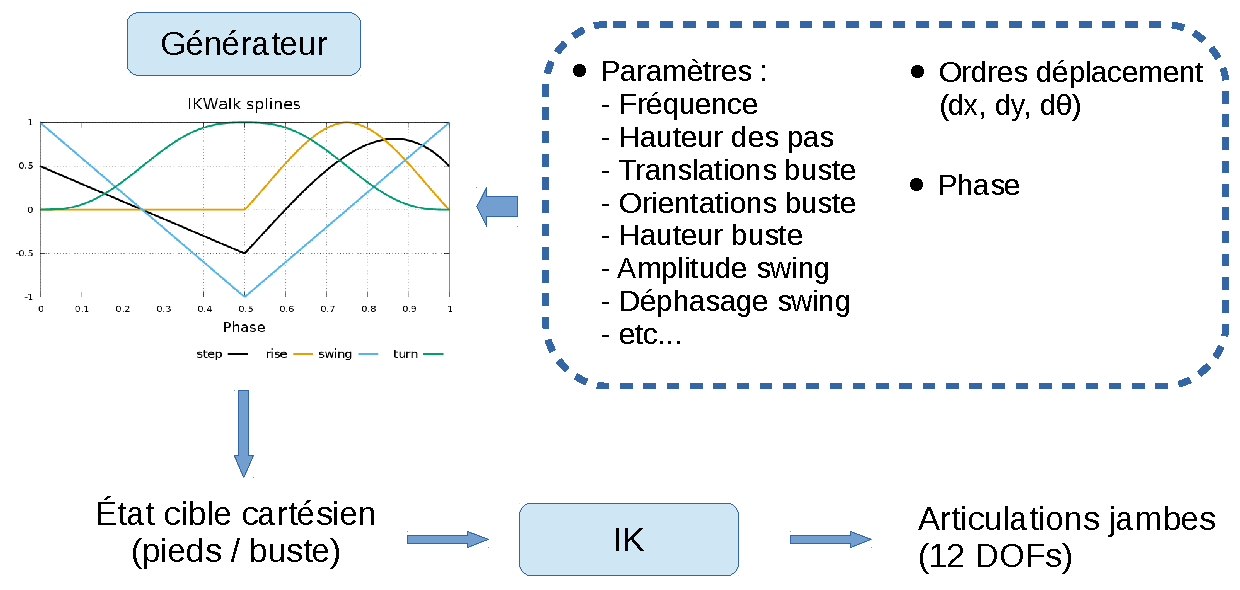
\includegraphics[type=pdf,ext=.pdf,read=.pdf,width=1.0\linewidth]{../schema/ikwalk}
        \caption{\label{fig:walk_schema} 
            Résumé du principe de fonctionnement du générateur de marche
            \textit{IKWalk}.
        }
    \end{center}
\end{figure}

\subsection{Ajustement des paramètres}

Voici les quelques principes généraux et commentaires appliqués lors 
du réglage expert des paramètres statiques (tableau \ref{tab:walk_params_static}) 
de la marche :
\begin{itemize}
    \item La fréquence propre du pendule inversé du robot est au alentour de $1$ Hz. 
        Néanmoins la fréquence de la marche \textit{freq} est toujours fixée 
        à une valeur plus élevée (entre $1.6$ et $1.7$ Hz).
        Ceci tend à améliorer la stabilité et à réduire les oscillations parasites.
        Une hypothèse pour expliquer ce phénomène fait intervenir le jeu mécanique
        des servomoteurs.
        Ce jeu en altère la dynamique du haut du corps de manière 
        semblable à un double pendule.
        Peut-être que des oscillations de marche plus hautes fréquences, 
        éloignées de la fréquence propre de ce pendule en haut du corps, 
        tendent à limiter ses perturbations.
    \item \textit{riseGain} est la hauteur à laquelle le robot lève ses pieds.
        Il est préférable de réduire cette valeur le plus possible afin de gagner
        en stabilité et d'éviter des mouvements amples inutiles au niveau des jambes.
        Sur de la moquette, une hauteur de $0.02$~m est suffisante. 
        Mais sur de l'herbe artificielle de plusieurs centimètres, il est nécessaire d'élever
        les pieds entre $0.03$ et $0.035$~m afin d'éviter tout frottement.
        Ceci tend à réduire la vitesse maximale atteignable sur herbe artificielle. 
    \item \textit{trunkZOffset} correspond à la hauteur (constante) du buste 
        du robot par rapport au sol. Plus le robot est haut, donc jambes tendues
        et moins la posture est difficile à maintenir et couteuse en terme
        de couples au niveau des genoux. Néanmoins, le mouvement de
        marche se base sur le contrôle des pieds (plats par rapport au sol) 
        en cartésien et donc sur le modèle géométrique inverse des jambes. 
        Augmenter la hauteur du buste du robot a pour effet de réduire l'espace cartésien 
        atteignable par le pied dans le plan sagittal. 
        Un compromis doit donc être trouvé entre
        la longueur maximale des pas et les efforts acceptables des servomoteurs.
    \item \textit{swingGain} et \textit{swingPhase} définissent l'amplitude et de décalage 
        temporel du mouvement de translation latéral gauche droite du buste 
        du robot par rapport aux pieds.
        Ce mouvement permet de déplacer alternativement le poids du robot d'un pied
        sur l'autre en coordination avec le décollage des pieds.
        Le décalage de phase, typiquement $0.25$ est en avance par rapport aux pieds
        car il prend en compte le retard de suivi de trajectoire des moteurs 
        et l'anticipation du transfert de poids.
        Le réglage cherche ici à assurer la stabilité latérale, notamment pendant 
        les pas chassés (latéraux) tout en essayant de minimiser les oscillations 
        latérales de la tête.
    \item \textit{trunkXOffset} et \textit{trunkPitchOffset} spécifient la position et 
        l'inclinaison du buste dans l'axe avant arrière du robot. 
        Ils permettent tous deux de contrôler le positionnement de la masse du haut du corps
        par rapport aux pieds. 
        Cette répartition de masse est importante étant donné que
        le robot tend à avancer vers l'avant lorsque l'on déplace la masse du haut 
        du corps vers l'avant des pieds\footnote{Ceci est encore dû aux imperfections 
        du contrôle proportionnel des moteurs dont le suivi de la consigne
        est fonction du couple externe appliqué sur le moteur.}.
        De plus, le buste s'incline vers l'arrière quand le robot augmente sa 
        vitesse de marche vers l'avant et inversement en marche arrière.
        Jouer à la fois sur la translation et sur l'inclinaison est essentiel
        pour obtenir une marche arrière fonctionnelle.
        Selon les robots, il peut être nécessaire d'avoir des réglages de 
        \textit{trunkXOffset} et \textit{trunkPitchOffset} différents pour la
        marche avant et la marche arrière. 
        Il peut également être utile pour améliorer la stabilité et la vitesse maximale 
        de mettre à jour continuellement ces deux paramètres proportionnellement 
        à la longueur des pas avant (\textit{stepGain}).
\end{itemize}

\subsection{Expérimentations et constats}

\begin{figure}[htb!]
    \begin{center}
        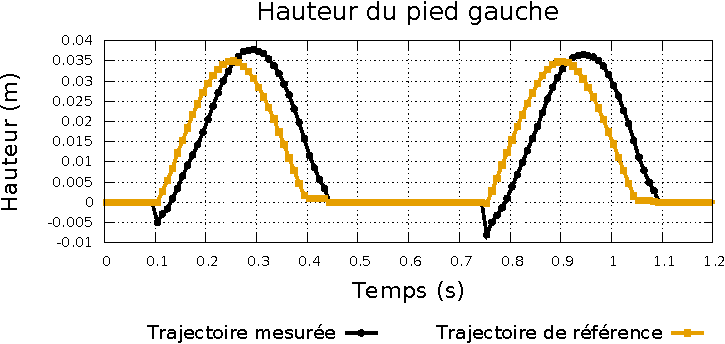
\includegraphics[type=pdf,ext=.pdf,read=.pdf,width=0.9\linewidth]{../plot/walk_time_foot}
        \caption{\label{fig:walk_time_foot} 
            Hauteur cartésienne dans le repère du monde 
            du centre du pied gauche (\textit{left\_foot\_tip})
            désirée générée par IKWalk 
            et mesurée sur le robot Sigmaban marchant vers l'avant.}
    \end{center}
\end{figure}

\begin{figure}[htbp]
    \begin{center}
        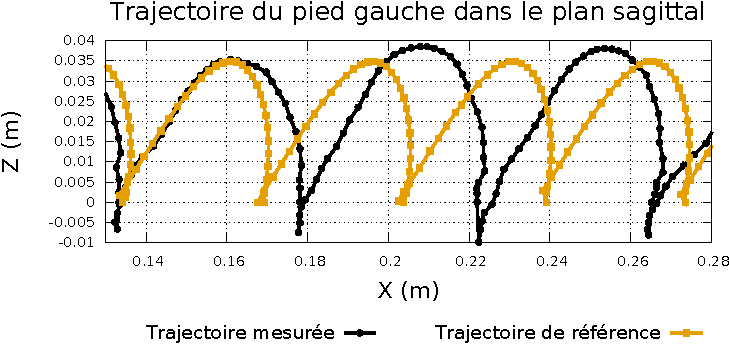
\includegraphics[type=pdf,ext=.pdf,read=.pdf,width=0.9\linewidth]{../plot/walk_traj_foot}
        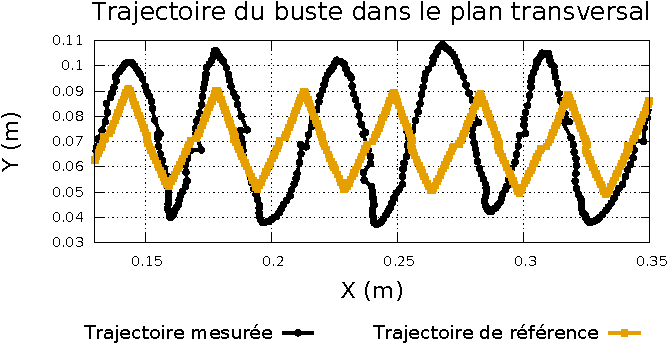
\includegraphics[type=pdf,ext=.pdf,read=.pdf,width=0.9\linewidth]{../plot/walk_traj_trunk}
        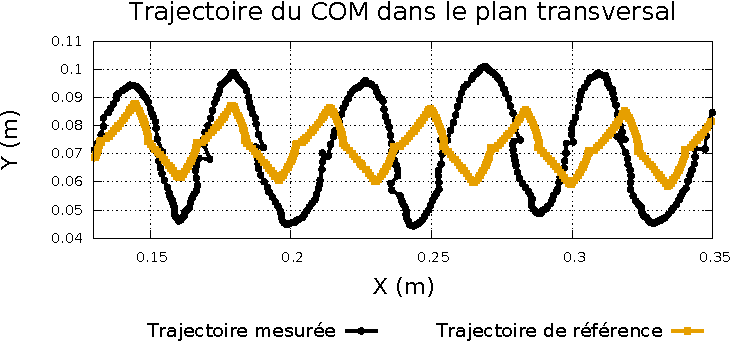
\includegraphics[type=pdf,ext=.pdf,read=.pdf,width=0.9\linewidth]{../plot/walk_traj_com}
        \caption{\label{fig:walk_trajs} 
            Comparaisons des trajectoires cartésiennes cibles générées par IKWalk 
            et mesurées sur le robot Sigmaban marchant vers l'avant
            du centre du pied gauche (\textit{left\_foot\_tip}), 
            du buste (\textit{trunk}) et 
            du centre de masse (\textit{COM}) dans le repère du monde.}
    \end{center}
\end{figure}

Les graphiques de la figure \ref{fig:walk_trajs} montrent les trajectoires de référence 
cartésiennes typiques générées par le générateur en boucle
ouverte pendant que le robot marche vers l'avant. 
De plus, les trajectoires effectivement réalisées par 
le robot sont reconstruites et dessinées grâce 
au modèle géométrique direct.
Enfin la figure \ref{fig:walk_time_foot} détaille les 
trajectoires de la hauteur du pied, cible et mesurée, en fonction du temps.

À noter que les petites discontinuités observées sur la trajectoire de référence
du buste et du centre de masse sont dues à l'accumulation des erreurs
numériques sur le modèle géométrique inverse des jambes.
Au moment du changement de pied de support, le pied sur le point de se poser
n'est pas parfaitement à hauteur nulle entrainant une discontinuité 
des positions cartésiennes.

On observe de manière générale sur les figures \ref{fig:walk_trajs} et
\ref{fig:walk_time_foot} une grande différence entre l'ordre en position 
envoyé aux moteurs et la trajectoire réellement suivie. Plus précisément :
\begin{itemize}
    \item La trajectoire mesurée possède un retard temporel par rapport 
        à la commande de l'ordre de $40$ ms. 
        Ce retard est variable et est le résultat du délai entre 
        le calcul de l'ordre désiré, la transmission de l'ordre au travers
        du bus série bas niveau, de la réaction mécanique des moteurs
        et enfin de la réception des mesures des encodeurs toujours sur le bus série.
        Pour rappel, la fréquence de la boucle de rafraichissement 
        en lecture et écriture bas niveau est de l'ordre de $100$~Hz.
        De plus, la fréquence de contrôle électronique
        du moteur est grande ($1000$~Hz) par rapport au retard considéré ici. 
        Le délai viens principalement de la méthode d'asservissement 
        purement réactive (proportionnel) du contrôleur et dépend du couple externe 
        appliqué sur le moteur.
    \item La longueur effective du pas réalisé est plus grande que voulue.
        Par exemple, si le pas désiré mesure $35$~mm (paramètre \textit{stepGain}), 
        le pas réel mesure entre $42$~mm et $45$~mm\footnote{La correction proportionnelle 
        calculée par apprentissage est en effet de l'ordre de 1.2 selon $\bm{\vec{x}}$.}.
        Ceci est dû d'une part, aux erreurs de suivi de trajectoire de l'asservissement
        réactif et proportionnel des moteurs, et d'autre part à l'accumulation de tous 
        les jeux mécaniques des articulations.
        Le jeu mécanique tend à augmenter avec l'usure des moteurs 
        et nuit fortement à la qualité d'asservissement
        de la trajectoire cible\footnote{Le jeu est ici \textit{mesuré} par les encodeurs 
        en sortie des palonniers des moteurs. Néanmoins, il induit une dynamique très 
        difficile à anticiper en plus que d'empêcher temporairement la transmission de 
        couple entre le moteur électrique et l'arbre de sortie.}.
    \item À noter que la forme complexe de la trajectoire désirée du centre de masse
        est calculée en prenant en compte toutes les masses dont le pied en vol.
        On peut également observer que la trajectoire mesurée du centre de masse 
        dans le plan transversal suit une oscillation qui n'est pas très éloignée 
        de la courbe théorique en sinus hyperbolique par morceaux donnée par 
        le pendule inversé de Kajita.
\end{itemize}
À noter également que l'on observe bien dans le plan sagittal la forme
de la trajectoire de référence du pied définie par les paramètres
\textit{stepUpVel}, \textit{stepDownVel}, \textit{riseUpVel} et \textit{riseDownVel}
affectant les tangentes au début et à la fin de la phase de levé du pied.

\subsection{Limitations\label{sec:walk_limitations}}

L'implémentation actuelle du générateur de marche fait appel à des splines cubiques.
L'utilisation de splines quintique (polynômes de degré cinq) permettrait une continuité
des accélérations et donc une trajectoire continue des couples 
et du \textit{Zero Moment Point} (ZMP).
De plus, les positions et orientations désirées des pieds sont
pour le moment exprimées dans le repère mobile du buste du robot. 
Il serait plus intuitif de les exprimer dans le repère fixe du pied de support 
même si cela introduit une discontinuité de la représentation au moment 
du changement de pied de support.\\

Au vu de ces limitations, un nouveau mouvement de marche, la \textit{QuinticWalk}
a été implémenté pour l'édition 2017 de la RoboCup.
Ce générateur reprend et corrige les points mentionnés ci-dessus.
La phase de double support est améliorée, la continuité jusqu'à
l'accélération de toutes les commandes des articulations est assurée.
Les oscillations latérales du haut du corps au démarrage et à la fin 
du mouvement sont spécialement traitées pour augmenter la stabilité.
Un contrôle du positionnement des pas du robot est rendu possible 
dans le repère fixe du pied de support courant.
Ce mouvement de marche utilisé en 2017 a notamment permis de grandement améliorer
la stabilité et la maniabilité du déplacement des robots expérimentaux 
de plus grandes taille, Grosban.
Ce générateur n'est pas détaillé dans ce manuscrit.
Cependant, son fonctionnement et le lien vers son code source sont rapidement
mentionnés à la section \ref{sec:other_works}.

\subsection{Validation du mouvement par le ZMP}

Comme mentionné ci-dessus, la trajectoire théorique du ZMP 
du mouvement \textit{IKWalk} n'est malheureusement pas continue,
et peut difficilement être utilisée pour valider le mouvement de marche.

Le mesure du ZMP sur le robot réel est quant à elle difficile.
Par définition, le ZMP est lié à l'accélération du centre de masse.
Avec le modèle géométrique direct et les différents capteurs, il est 
possible d'estimer la position du COM. 
Malheureusement, cette estimation est directement affectée par
la somme du bruit des encodeurs et de la centrale inertielle.
La différentiation numérique jusqu'à l'accélération de cette 
estimation bruitée n'est pas proprement réalisable.
Les travaux sur la marche des petits robots humanoïdes NAO (\cite{graf_center_2011})
se basent bien sur un filtre de Kalman pour estimer la vitesse du COM, 
mais pas son accélération.

Enfin, il serait possible d'employer les capteurs de pression du robot,
mesurant une estimation du centre de pression (\cite{PassaultThesis}).
Ce dernier est confondu avec le ZMP tant qu'il n'atteint pas
la bordure des pieds (roulement).
L'étude de l'utilisation des capteurs de pression pour l'estimation
en temps réel du ZMP du robot reste à entreprendre.\\

\begin{figure}[htb]
    \begin{center}
        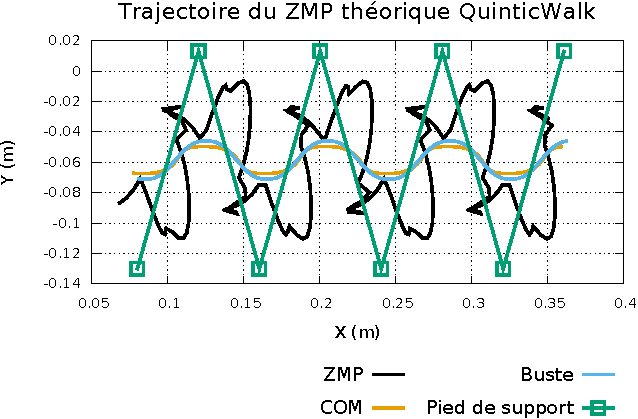
\includegraphics[type=pdf,ext=.pdf,read=.pdf,width=1.0\linewidth]{../plot/walk_quintic_zmp}
        \caption{\label{fig:walk_quintic_zmp} 
            Trajectoires théoriques de commande du ZMP, du buste et du centre de masse de Sigmaban.
            Le robot marche tout droit en utilisant le générateur de marche \textit{QuinticWalk}.
            Les paramètres du générateur sont ceux employés lors de l'édition 2017 de la RoboCup.
            Le ZMP est calculé au travers du modèle dynamique inverse du robot.
            Les trajectoires sont représentées du dessus dans le plan transversal.
        }
    \end{center}
\end{figure}

Sur la nouvelle marche \textit{QuinticWalk}, le calcul de
la trajectoire continue du ZMP est possible et est représentée
sur la figure \ref{fig:walk_quintic_zmp}.
On remarque tout d'abord que la forme de cette trajectoire théorique 
est bien plus complexe et imprécise que la trajectoire en \og créneaux \fg 
générée par les méthodes de Kajita.
La forme générale est cependant bien respectée.
À noter que contrairement aux travaux classiques se basant
sur le modèle du pendule inversé, ici, 
l'intégralité de la dynamique est prise en compte (par exemple, l'influence
de la deuxième jambe en vol).
Deuxièmement, l'amplitude des oscillations du ZMP est inférieure
à la distance d'écartement latérale ($Y$) des pieds.
En théorie, le ZMP est sensé atteindre la position latérale du centre 
des pieds pour garantir la stabilité du robot.
Or, comme expliqué à la section \ref{sec:robot_flaws}, le jeu mécanique et les
défauts d'asservissement tendent à augmenter les amplitudes de toutes les oscillations.
De plus, les paramètres de la marche utilisés ici ont été manuellement ajustés 
sur le robot réel dans le but de maximiser sa stabilité et sa vitesse.
Sur la base de la robustesse effective de la marche, 
on peut ainsi faire l'hypothèse que sur le robot physique, les imperfections 
(pris en compte implicitement dans le réglage des paramètres) font que 
la trajectoire réelle du ZMP atteint bien le centre des pieds.

\subsection{Méthode de stabilisation\label{sec:walk_stabilization}}

\begin{figure}[htb!]
    \begin{center}
        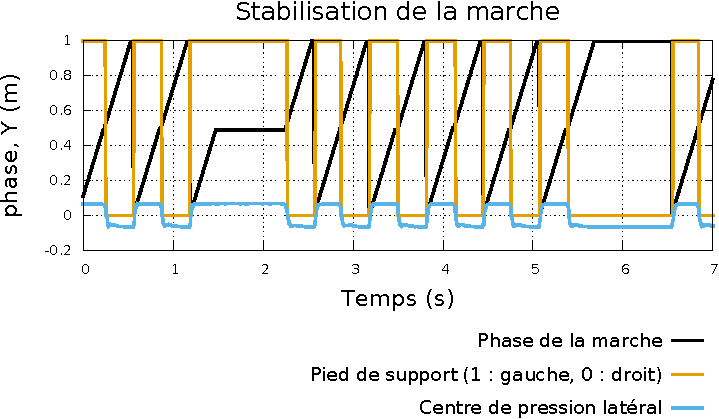
\includegraphics[type=pdf,ext=.pdf,read=.pdf,width=0.9\linewidth]{../plot/walk_stabilization1}
        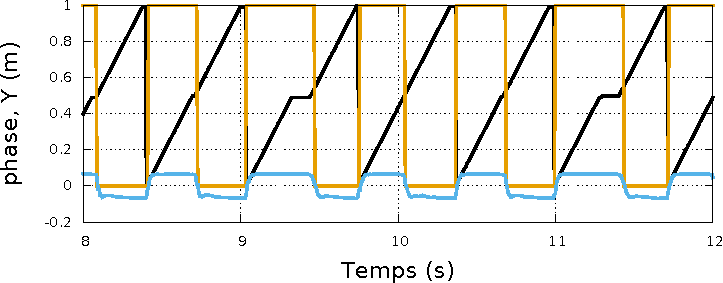
\includegraphics[type=pdf,ext=.pdf,read=.pdf,width=0.9\linewidth]{../plot/walk_stabilization2}
        \caption{\label{fig:walk_stabilization} Stabilisation de la marche par
            pause du mouvement aux phases $0$ et $0.5$ selon la mesure du centre de pression
            latéral. Le robot Sigmaban marche sur place. 
            À $t \approx 1.4$~s, le robot est maintenu manuellement sur son pied gauche.
            À $t \approx 5.6$~s, le robot est maintenu manuellement sur son pied droit.
            Enfin, à $t \approx 9.3$ et $11.3$~s, le robot est impacté sur son flanc droit.
        }
    \end{center}
\end{figure}

Le générateur de mouvement en boucle ouverte \textit{IKWalk} présenté précédemment 
est associé avec une technique de stabilisation simple 
améliorant la robustesse de la marche.
Cette stabilisation n'intervient que dans le plan latéral.
Il s'avère en pratique que l'ajustement manuel des paramètres statiques 
du mouvement permet d'assurer une stabilité avant arrière acceptable.
La stabilité latérale est en effet comme l'explique Marcell Missura dans son 
article \cite{missura_lateral_2011}, fondamentalement plus délicate à contrôler que la 
stabilité dans le plan sagittal.
Si le centre de masse du robot dépasse latéralement la verticale
d'un des pieds, le robot se met à rouler sur les arrêtes de son pied et à tomber. 
Chez l'humain, seule une réaction rapide de saut ou le croisement des jambes permet
de recouvrir la stabilité bipède. Cette manœuvre étant très difficile voire impossible
géométriquement à accomplir sur nos petits robots, cette situation est à éviter autant
que possible.
De plus, il s'avère que la stabilité latérale est particulièrement mise en défaut 
par les pas latéraux, nécessaires pour avoir la marche omnidirectionnelle. 
Typiquement sans stabilisation, on observe que les pas chassés font parfois
entrer la dynamique du robot dans une oscillation entretenue d'un pied 
sur l'autre entrainant au bout de deux ou trois pas sa chute.

Cette méthode de stabilisation a été mise au point par Grégoire Passault
et est étudiée en détail dans ses travaux de thèse \cite{PassaultThesis}.
Il s'agit de \og mettre en pause \fg le mouvement à certains 
points de la phase si la position du centre de pression latéral mesurée par 
les capteurs des pieds est en dehors d'un certain intervalle.
L'intuition dernière cette méthode est d'éviter de lever un
pied si le poids du robot n'a pas encore été déplacé sur l'autre pied.

Plus en détail, une moyenne pondérée sur les mesures de pression des deux pieds
permet d'évaluer la position du centre de pression global
$\bm{p}_{\text{CoP}} \in \mathbb{R}^{2}$ sur le sol et dans le repère 
égocentrique du robot.
Ensuite, le seuil de déclenchement de la stabilisation est définie par le paramètre 
\textit{securityThreshold}~$\in [0,0.1]$ représentant la largeur en mètre de l'intervalle latéral
admissible pour la position du centre de pression.
Au moment du changement du pied de support 
(phase à $0$ et $0.5$)\footnote{La notion d'égalité sur la phase du mouvement, par exemple 
$\varphi_{t} = 0.5$ est en pratique à remplacer par la vérification 
de la transition $\varphi_{t-1} < 0.5$ et $\varphi_{t} \geqslant 0.5$.},
le mouvement est mis en pause (phase constante) si le centre de pression n'est pas 
dans l'intervalle admis \footnote{Si $\varphi_{t} = 0.5$, le pied gauche est sur le point de décoller. 
Donc si le centre de pression $\bm{p}_{\text{CoP}}.\bm{\vec{y}} > \text{\textit{securityThreshold}}$
est trop loin sur la gauche du robot, mieux vaut ne pas lever le pied} :

$$
\text{Si }
\begin{cases}
    \varphi_{t} = 0.0 \text{ \textbf{et} } \bm{p}_{\text{CoP}}.\bm{\vec{y}} < -\text{\textit{securityThreshold} \textbf{ou}}\\
    \varphi_{t} = 0.5 \text{ \textbf{et} } \bm{p}_{\text{CoP}}.\bm{\vec{y}} > \text{\textit{securityThreshold}}\\
\end{cases}
\text{ alors }
\varphi_{t+1} = \varphi_{t}
$$

La figure \ref{fig:walk_stabilization} illustre le processus de stabilisation.
En cas d'impact sur le robot du coté droit (à $t \approx 9.3$~s), 
la position du centre de pression latéral reste alors plus longtemps sur
le pied gauche (environs $380$~ms contre $250$~ms normalement) traduisant
un déséquilibre temporaire. 
La marche est alors stoppée pendant environs $110$~ms.

On remarque que même sans perturbation extérieure, la stabilisation s'active et
temporise la marche durant une courte période de l'ordre de $20$~ms 
au début de chaque phase de support. Il est intéressant de constater que cette
temporisation tend à augmenter quand la fréquence de la marche diminue. 
Par exemple, il est possible d'atteindre une fréquence de marche plus anthropomorphique 
de l'ordre de $1$~Hz stable ce qui est très difficile en boucle purement ouverte. 
Les temporisations de la marche y sont alors importantes.

À noter que Grégoire Passault a dans son document de thèse 
(\cite{PassaultThesis}) proposé une amélioration de cette 
méthode en apprenant le profil nominal des mesures des capteurs.
Cette technique n'est cependant pas employée ici lors des expérimentations 
sur l'odométrie.\\

Au final, l'ajout d'une stabilisation simple en boucle fermée améliore
la robustesse de la marche.
Néanmoins, cette procédure affecte le déplacement du robot et du point de vu
du modèle de déplacement, prévoyant le comportement du robot sans lecture
des capteurs, l'activation de la stabilisation doit être vu comme un bruit
affectant potentiellement les pas du robot.
De plus, le robot est d'autant moins stable que les ordres d'avance ou de pas
chassés sont grand. La stabilisation se déclenchant donc plus souvent.
Il est ainsi a priori important pour le modèle de déplacement 
de considérer un bruit dépendant des ordres de la marche.

